\newcommand{\java}{Java 8}
\newcommand{\mavenLarge}{Apache Maven 3.6.3}
\newcommand{\maven}{\texttt{maven} }
\newcommand{\ciglib}{\texttt{CigLib} }
\newcommand{\toml}{\texttt{Toml}}
\nc{\dto}{\texttt{DTO} }
\nc{\factoryDTO}{\texttt{FactorySMSDatagram} }

\begin{document}
\section{Anàlisis de requisits}
Des d'un punt de vista general, al voler realitzar una simulació, els requisits del projecte no tenen la projecció d'un entorn realista, ja que l'objectiu és dur a terme un anàlisis dels costos empírics del projecte, com per exemple, veure on està el coll d'ampolla o mesurar i poder parametritzar els valors més idonis pel protocol.
\\
\\
En més concret, s'han trobat els següents requisits:
\begin{itemize}
	\item Des del punt de vista d'arquitectura de xarxa, es pot veure clarament que el model es pot definir com client-servidor, ja que la interacció entre les diferents entitats és centralitzada.
	\item És important mantenir el codi més obert possible per tal de realitzar els canvis de la manera més còmode, sobretot en els següents apartats: la connexió entre els clients i el servidor i la incorporació de diferents criptosistemes per realitzar el xifratge.
	\item S'ha de tenir en consideració el llenguatge i les eines a utilitzar per tal de facilitar la lògica.
	\item S'ha d'intentar tenir la capacitat de realitzar els canvis sobre les diferents paquets i llibreries en cas que es necessiti.
	\item Un cop creada la implementació, s'ha de poder realitzar un anàlisis de costs el més detallat possible.
	\item El sistema tant pel punt de vista del comptador com per la subestació ha de ser totalment configurable. És a dir, s'ha de passar per paràmetre la configuració del protocol explicada en la secció \ref{sec:configuracio-recsi}.
\end{itemize}
\subsection{Característiques tècniques}
La simulació del projecte s'ha implementat utilitzant \texttt{\java} i \texttt{\mavenLarge} per la gestió de paquets. La inclinació per utilitzar \texttt{\java} és degut a la llibreria \ciglib creada per Víctor Mateu, que recopila implementacions tant de sistemes criptogràfic com de funcions hash, entre altres. D'aquesta forma, s'intenta assolir el màxim els requisits detallats anteriorment.
\\
\\
A l'utilitzar \maven per la gestió de paquets i dependència, s'ha canviat la estructura de la llibreria i s'ha pujat a un repositori remot \cite{ciglib}. Per instal·lar-la només cal configurar el servidor de \texttt{GitHub} a \maven i cridar la dependència al projecte que es vulgui.
\\
\\
Per realitzar la configuració, s'ha decidit utilitzar el format \toml\footnote{Format de fitxer per a fitxers de configuració.} ja que és fàcil i ràpid de llegir i d'escriure a causa de la seva sintaxis i semàntica minimalista i està dissenyat per transformar sense ambigüitats el fitxer a un diccionari.
\section{Disseny}
El projecte es divideix en un total de \numitems{list:packages} paquets que s'encarreguen de diferents responsabilitats.
\begin{itemize}
	\item \texttt{connection} s'encarrega d'aportar la connexió entre els comptadors i la subestació, carregant d'aquesta manera els diferents \textit{datagrames} o  \texttt{Data Transfer Objects} (\texttt{DTO}).
	\item A \texttt{busom} hi ha la implementació de \cite{busom}.
	\item \texttt{consumption} es responsabilitza de rebre les lectures de consum d'energia.
	\item A \texttt{recsi} s'hi trobarà la implementació de la proposta \cite{recsi}.
	\item Al paquet \texttt{main} hi ha les diferents classes on s'inicia l'aplicació. \label{list:packages}
\end{itemize}
\subsection{Configuració}
La configuració del sistema i de cada entitat (sigui comptador o subestació ) ve donada per dos fitxers:
\begin{itemize}
	\item Fitxer de configuració del sistema, que serà compartit per totes les entitats del barri, ja que inclourà:
	\begin{itemize}
		\item La corba el·líptica.
		\item El punt generador de la corba.
		\item El cos primer de la corba.
	\end{itemize}
	Les dades d'aquest fitxer estaran encapsulades a la classe \texttt{CurveReader}, que funcionarà com una \texttt{dataclass}\footnote{Classe que només té la responsabilitat d'encapsular informació.}.
	
	\item Fitxer de configuració de xarxa, on vindrà donada la direcció $ip$ del servidor i el seu port on escoltarà. D'aquesta manera, la subestació, donada aquesta configuració crearà un \texttt{ServerSocket} per escoltar en el port i cada comptador crearà un \texttt{Socket} que estarà enllaçat al socket del servidor.
\end{itemize}
\subsection{Connexió}
En \texttt{connection} trobem 3 interfícies que representen les diferents responsabilitats del paquet:
\begin{itemize}
	\item \texttt{ReceiverMeter }s'encarrega de rebre el \dto de la subestació.
	\item \texttt{ReceiverSubestation }rebrà tots els \dto dels comptadors.
	\item \texttt{Sender }només s'encarregarà d'enviar \dto ja sigui de part d'un comptador o de la subestació.
\end{itemize}
La implementació d'aquestes interfícies s'ha realitzat usant les classes \texttt{Socket} i \texttt{ServerSocket} de \texttt{java.net} pels comptadors i la subestació respectivament.
\subsubsection{Data Transfer Objects}
Al haver de realitzar enviaments amb diferent contingut, s'han creat 5 datagrames, com es pot observar a la \textit{Figura \ref{fig:dto}}. En cada una de les classes s'ha usat el patró \textit{abstract factory} per serialitzar-los. S'ha realitzat una interfície anomenada \factoryDTO on cada implementació incorporarà la serialització del seu respectiu datagrama.
\begin{figure}[H]
	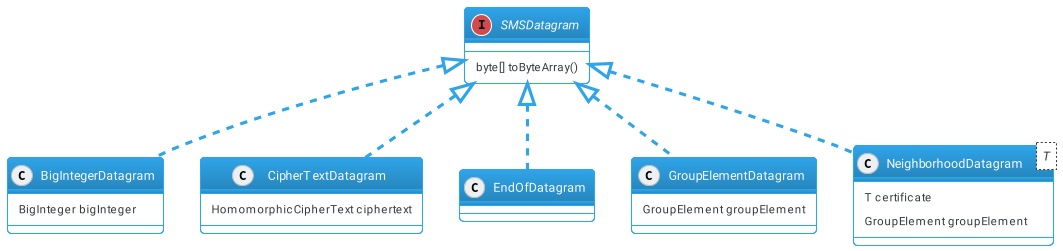
\includegraphics[width=15cm]{classes/dto.png}
	\caption{Diagrama de classe dels DTO}
	\label{fig:dto}
\end{figure}
% TODO DTO umls
\subsection{Criptografia}
A l'hora de fer una primera iteració sobre el projecte, es va veure clar crear una capa entre \ciglib i el sistema, d'aquesta manera, s'intenta satisfer el requisit de mantenir el codi més obert possible per a possibles futurs canvis. A fi de realitzar-ho, s'han creat interfícies, les implementacions les quals aporten la lògica de xifrar i desxifrar.
\subsubsection{CigLib}

\subsubsection{Integració al projecte}
 Per tal d'habilitar altres criptosistemes que no siguin ElGamal, s'ha usat el patró \texttt{strategy} i d'aquesta manera, només caldrar implementar una nova classe i passar-li pel constructor el nou criptosistema per modificar el comportament.
%TODO S'ha de fer
\subsection{Patró Màquina-Estat}
Per tal de crear una lectura entenedora dins de la complexitat del protocol, es va pensar en implementar-lo utilitzant el patró de disseny \texttt{Màquina-Estat}. L'avantatge d'utilitzar aquesta arquitectura de disseny davant de les altres és l'analogia que comparteix amb diagrames de flux o d'estat, cosa que permet implementar algoritmes complexos de manera més senzilla. \texttt{Màquina-Estat} resumeix tota la lògica relativa als estats i a les transicions, és a dir, ens podrem estalviar condicionals i problemes de complexitat de lectura en el codi.
\\
\\
Aquest patró consisteix en tenir una interfície \textit{Estat} amb el mètode \textit{next}, que retornarà el nou \textit{Estat} donat el context de l'aplicació. És important tenir en consideració que el treball a realitzar dels comptadors i de la subestació serà diferent i, per tant, la implementació dels estats no es compartirà. D'aquesta manera, el punt o estat del programa estarà determinat pels tipus d'\textit{Estat} que estan la subestació com els comptadors en aquell moment. Gràcies a això, creant unes validacions i precondicions adequades, la màquina d’estat impedeix operacions fora del nostre entorn.
\\
\\
No obstant això, aquest tipus d'arquitectura també té inconvenients. Un d'ells és que la seva rigidesa impedeix crear una bona estructura per projectes que necessiten molta asincronia. Per sort, el nostre protocol es el suficientment rígid per no permetre accions d'asincronia, és més, l'implementació es quedarà beneficiada d'aquesta rigidesa.
\subsubsection{Implementació en RECSI i Busom}
En \texttt{recsi}, el context ve donat per les classes \texttt{SubstationContext} i \texttt{MeterContext}, on hi haurà la configuració i les dependències relatives a la connexió.
\\
\\
\end{document}
